\chapter{Análise Bibliográfica sobre Simulação Multiagente no contexto de Incêndios Florestais, por Gabriel Pinheiro\label{chap:bibliometria:pinheirogh}}

\section{Planejamento do estudo\label{pinheirogh:questoes}}
Muito tem sido pesquisado acerca da preservação de grandes áreas de vegetação em diversos países mundialmente. A quantidade de artigos chega a números estratosféricos em simples pesquisas por termos chaves em uma base de dados grande, como por exemplo a Web Of Science (WoS). Por isso, faz-se necessária a definição de questões norteadores ou focais, de modo a refinar a busca por artigos que apresentem maior compatibilidade com a área de estudo que se planeja analisar.

Para essa análise, as questões focais definidas foram as seguintes:
\begin{itemize}
    \item Como tem sido desenvolvidas pesquisas que usam simulação computacional para investigar o comportamento de incêndios florestais?
    \item Quais países têm sido referência na pesquisa mundial em relação aos incêndios florestais?
    \item Há relação entre a vegetação, bioma, clima e consequente quantidade de incêndios dos países referência e a quantidade de pesquisas que esses produzem na área referida?
    \item Quais as variáveis dependentes e independentes aparacem com mais frequência nas pesquisas?
\end{itemize}

\subsection{Uso do Bibliometrix e Biblioshiny}
Serão usadas a ferramenta e o \textit{workflow} proposto pelos autores do pacote Bibliometrix, conforme indica a figura ~\ref{fig:bibliometrix:workflow}.


\section{Coleta de dados\label{pinheirogh:coleta}}

A coleta de dados foi feita usando a WoS no dia 04 de dezembro de 2022, acessado por meio do Portal de Periódicos da CAPES.

\subsection{Query de Busca}

Foi usada a \query\  de busca ilustrada nas linhas 1 a 9 da listagem \ref{querypinheirogh2022-2}.

\lstinputlisting[numbers=left,basicstyle=\normalsize\ttfamily,caption={\query\  de busca sobre simulação agente/multiagente no contexto de incêndios florestais.},label=querypinheirogh2022-2]
{exploratory-data-analysis/pinheirogh/PesqBibliogr/ForestFire/query.txt}

\subsubsection{Explicação para os termos de busca usados\label{pinheirogh:query}}

A busca consistiu de quatro cláusulas disjuntivas, unidas por uma conjunção \textit{and}, aplicadas à busca por tópico (O termo de busca pode aparecer no Título, no Abstract, na Author Keywords, ou nas Keywords Plus da referência)

O termo / cláusula  \texttt{simul*}, na linha 1, foi usado em conjunção com os demais para recuperar apenas trabalhos que explicitem o uso da simulação.
Foi usado um único termo devido à forte adesão ao termo simulação por parte dos pesquisadores que usam simulação. Não existem outros sinônimos frequentes para esse uso.

A cláusula na linha 3 faz união entre o uso dos termos \texttt{agent} e \texttt{multiagent}, para cobrir as variadas formas de escrita do conceito.

A cláusula na linha 5 faz a junção de variados termos que na query buscam fazer o papel de adjetivo. Os termos geralmente especificam o tipo de incêndio que se pretende analisar. Essa cláusula é a mais importante da query já que é através dela que os termos, \texttt{forest fire}, \texttt{bushfire} e \texttt{wildfire}, considerados de grande valor para o foco desta análise, podem aparecer.

A negação presente na linha 8 e a cláusula presente na linha 9 possuem como objetivo a tarefa de eliminar artigos não relacionados ao foco desta análise. As cláusulas anteriores retornam muitos artigos em áreas relacionadas ao estudo de vivência de animais específicos como lobos, peixes, ovelhas e ursos. E ainda, artigos relacionados aos estudo de comportamento de consumidores e produção de energia renovável. Desse modo, os termos escolhidos excluem esses artigos do \textit{dataset} e melhoram a qualidade da análise. 

\subsection{Registros recuperados}

Os 239 registros obtidos como resultado da busca encontram-se em \url{https://github.com/jhcf/Comput-Experim-20222/blob/main/exploratory-data-analysis/pinheirogh/PesqBibliogr/ForestFire/query.txt}.

Foram utilizadas as opções \textit{Exportar registros para arquivo de texto sem formatação} e \textit{export full record / Gravar Conteúdo: Seleção personalizada, com todos os 29 campos disponíveis, inclusive referências citadas} no WoS, para que as citações também fosse usadas em análises da citações (estrutura intelectual do conhecimento). Os 239 registros foram recuperados em cinco blocos de até 50 registros por vez.


\section{Análise dos dados\label{MASSA@jhcf:analise}}


\subsection{Análise descritiva do \dataset}
Para buscar respostas às perguntas focais, diversos gráficos foram retirados da análise do \textit{dataset} através da ferramenta Bibliometrix/Biblioshiny.


A análise do primeiro gráfico proposto (figura \ref{fig:a}) revela que a produção científica acerca do tema de Incêndios Florestais têm crescido nos últimos 20 anos. Em alguns países, esse crescimento é consideravelmente grande se comparado a outros países no mesmo período de tempo, como é o caso dos Estados Unidos.

De acordo com XXX (Inserir citação a cerca da extensao da vegetação dos Estados unidos) e ainda de acordo com XXX (Inserir citação a cerca das frequencias das queimadas nos Estados Unidos). Isso pode tornar mais simples a compreensão do crescimento nessa área de pesquisa do país em questão.

Deste mesmo gráfico percebe-se também curva acentuada de crescimento para o país Canadá que geograficamente possui vegetação similar à dos Estados Unidos.

Analisando-se o gráfico \ref{fig:a} juntamente com o gráfico \ref{fig:e} fica clara também a relação de proximidade regional dos países líderes na pesquisa mundial deste tópico. O gráfico \ref{fig:e} evidencia ainda 2 outros países de grande relevância para a pesquisa recortada pelo \textit{dataset}: China e Australia.

De acordo com XXX (Inserir referências relacionadas à vegetação e queimadas da China) E ainda de acordo com XXX (Referências relacionadas à vegetação e queimadas da Australia)

Já o gráfico \ref{fig:d} evidencia como tem sido desenvolvida a pesquisa na área Incêndios Florestais. Através dos \textit{clusters} de cor vermelha e azul fica claro que os métodos de pesquisa utilizados pelos autores do \textit{dataset} incluem principalmente simulações que pretendem analisar o comportamento dos fenômeno através de modelos pré estabelecidos  

Ainda do gráfico \ref{fig:d} e agora inserindo à analise os gráficos \ref{fig:b} e \ref{fig:d} pode-se extrair as principais variáveis dependentes e independentes em foco nas pesquisas, com especial atenção ao termo ``Climate-change'' \footnote{Mudanças Climáticas} que de acordo com o gráfico \ref{fig:d} apresentou acentuada ascenção a partir do ano de 2014. Tal caracteristica pode ser explicado pelos dizeres de XXX nos quais ele apresenta os seguintes fatos: (Inserir citação que evidencia 2014 como ano mais quente dos registros modernos mundiais). Sabe-se de comum acordo que o fator temperatura mundial ambiental é uma grande variável dentro dessa área de pesquisa.

Outras variáveis que podem ser extraídas dos gráficos analisados são relacionadas abaixo:
\begin{itemize}
    \item Growth
    \item Spread 
    \item Tree mortality
    \item Carbon emission
\end{itemize}

\begin{figure}[H]
    \centering
    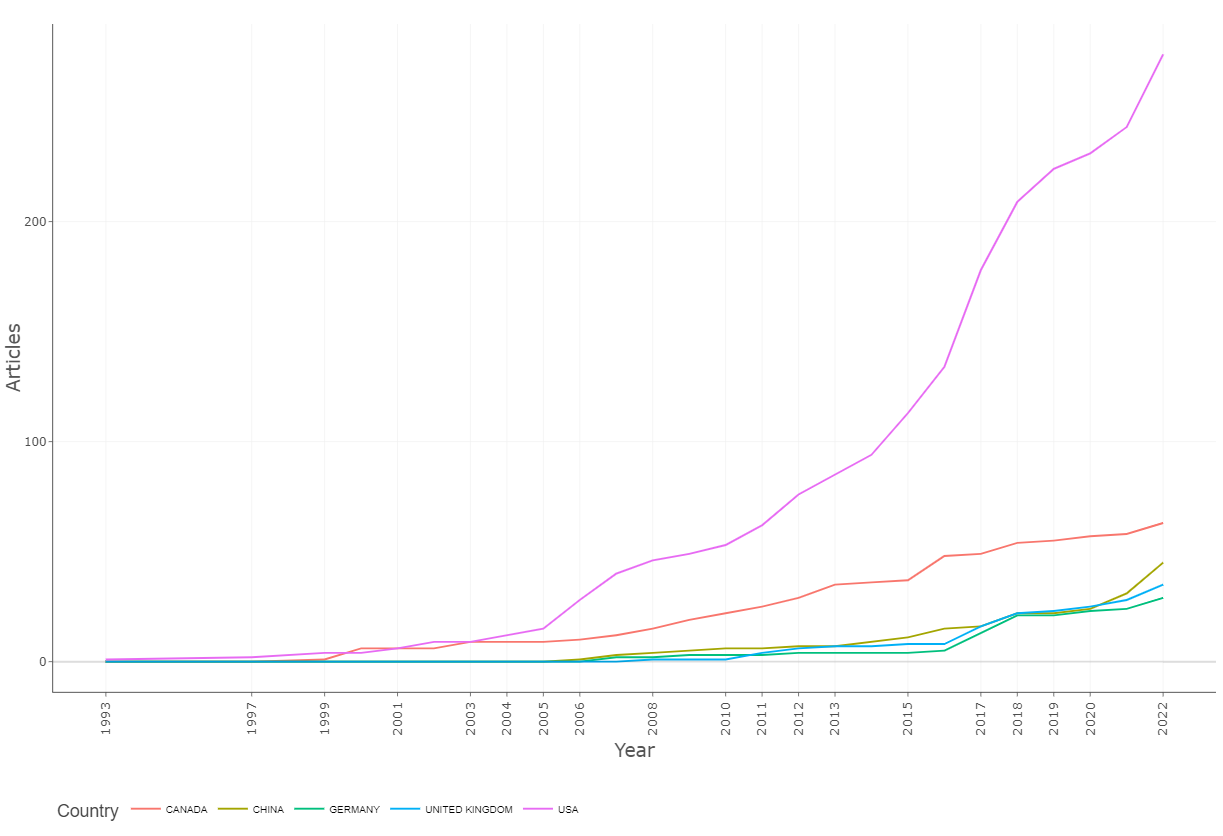
\includegraphics[width=1\textwidth]{exploratory-data-analysis/pinheirogh/PesqBibliogr/ForestFire/Gráficos/ProducaoCientifica.png}
    \caption{Evolução da produção científica no \textit{dataset}}
    \label{fig:a}
\end{figure}

\begin{figure}[H]
    \centering
    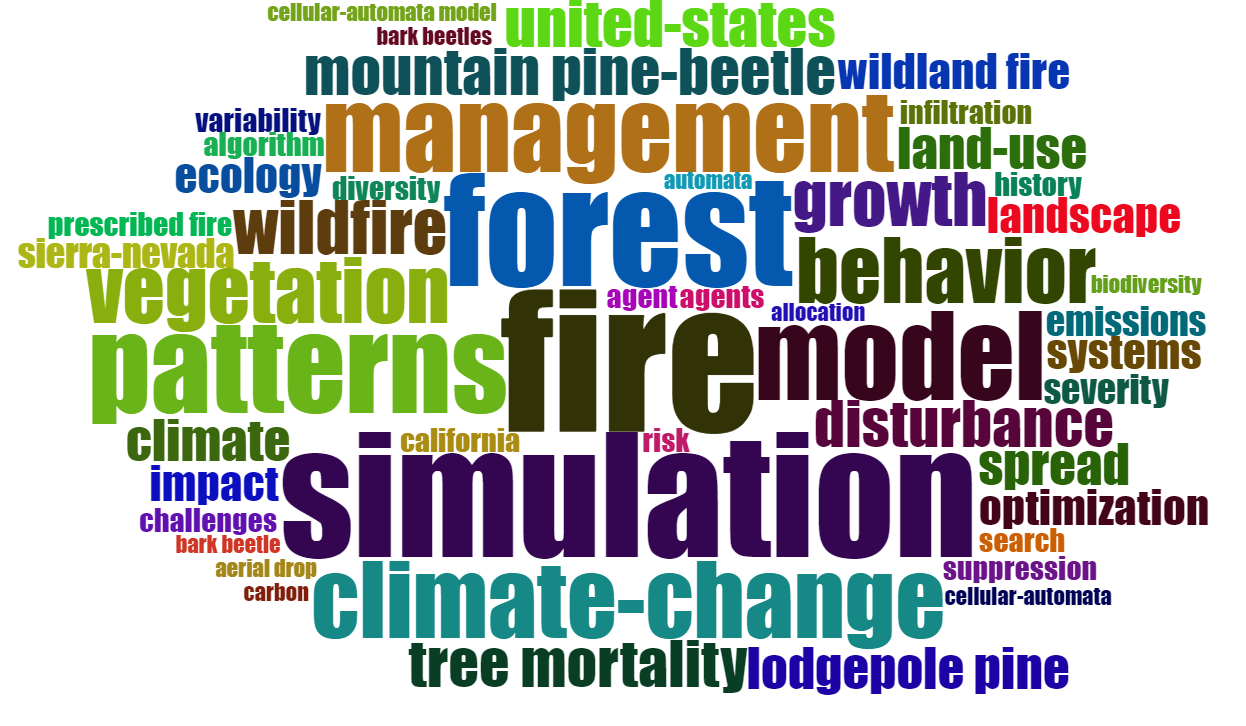
\includegraphics[width=1\textwidth]{exploratory-data-analysis/pinheirogh/PesqBibliogr/ForestFire/Gráficos/NuvemPalavras.png}
    \caption{Nuvem de Palavras no \textit{dataset}}
    \label{fig:b}
\end{figure}

\begin{figure}[H]
    \centering
    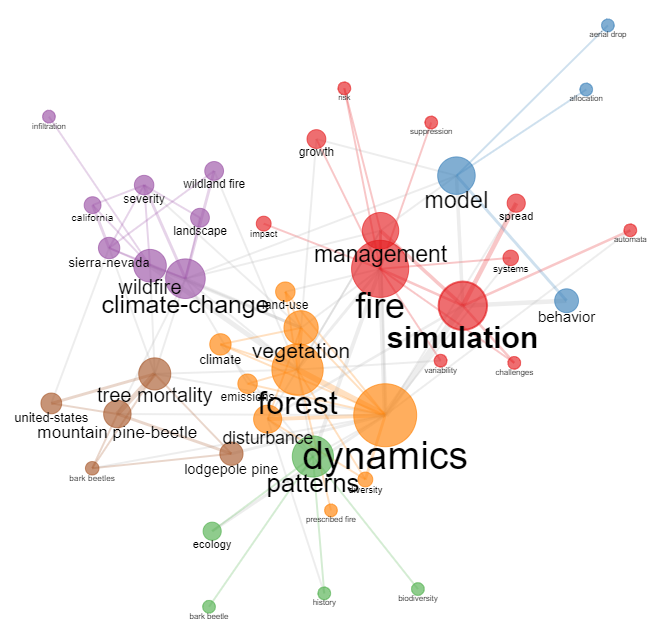
\includegraphics[width=1\textwidth]{exploratory-data-analysis/pinheirogh/PesqBibliogr/ForestFire/Gráficos/Network.png}
    \caption{Relacionamentos entre os termos mais citados}
    \label{fig:d}
\end{figure}

\begin{figure}[H]
    \centering
    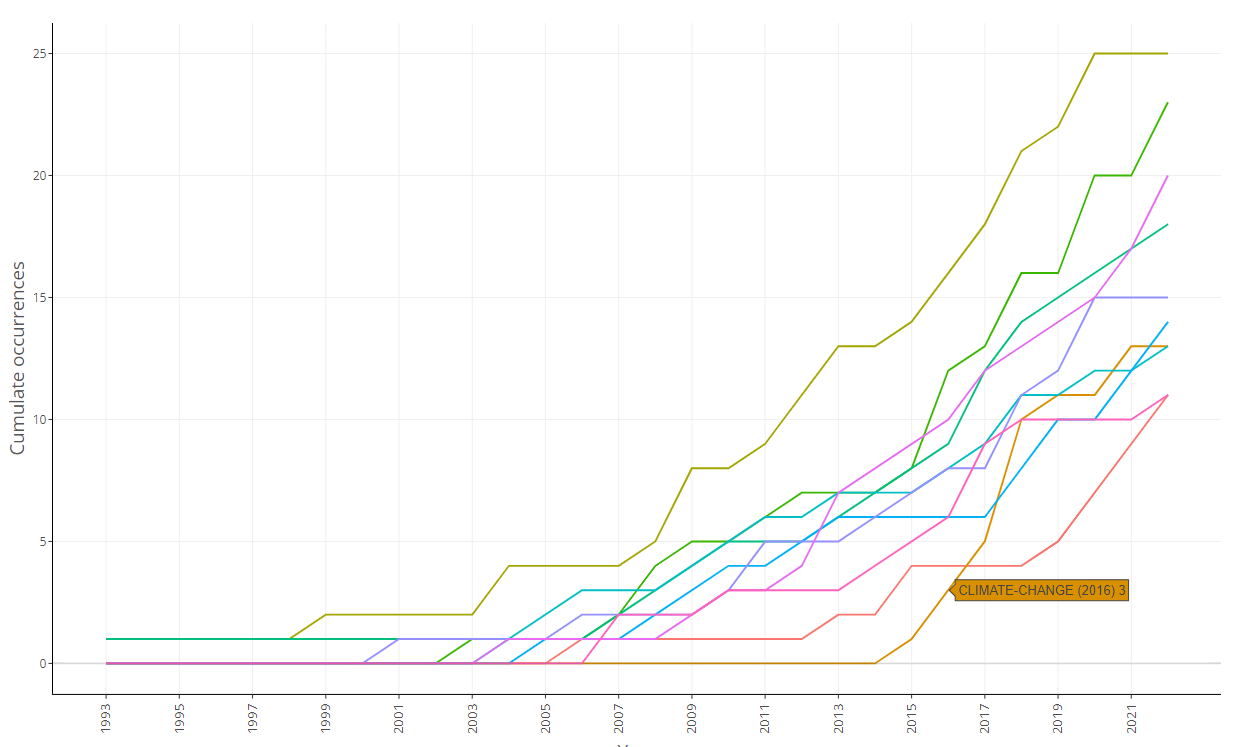
\includegraphics[width=1\textwidth]{exploratory-data-analysis/pinheirogh/PesqBibliogr/ForestFire/Gráficos/ClimateChangeOccurrences.png}
    \caption{Ascensão do termo ``Climate Change'' no \textit{dataset} ao longo dos anos}
    \label{fig:d}
\end{figure}

\begin{figure}[H]
    \centering
    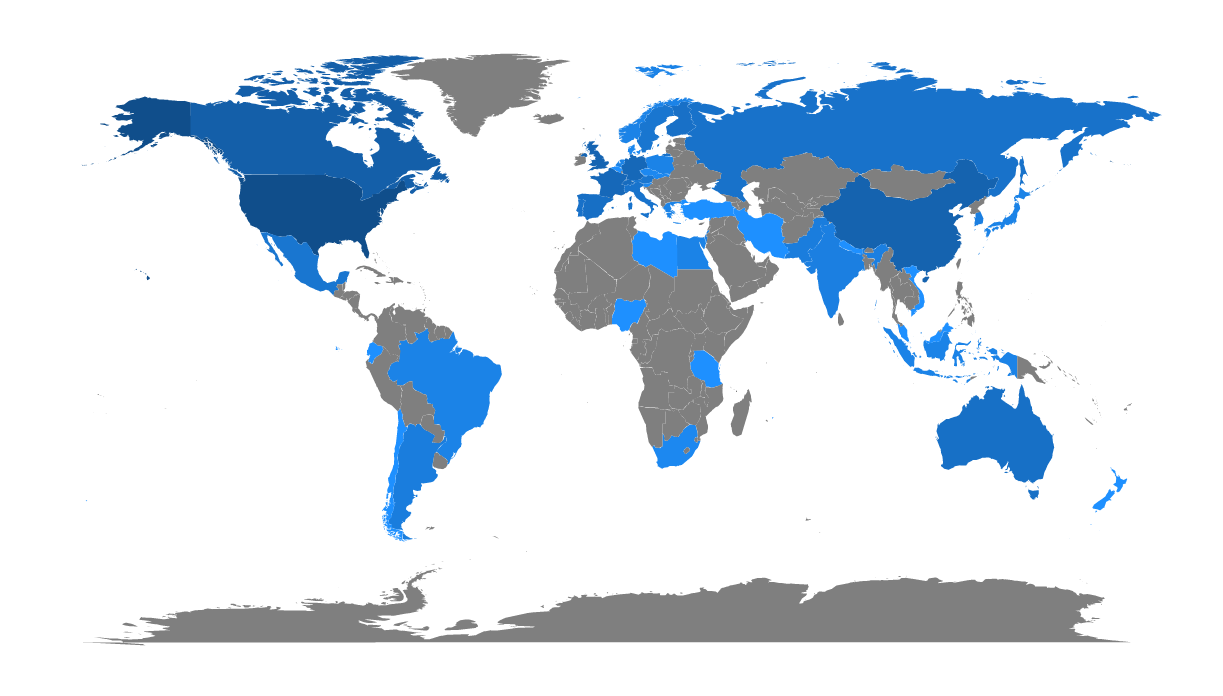
\includegraphics[width=1\textwidth]{exploratory-data-analysis/pinheirogh/PesqBibliogr/ForestFire/Gráficos/WorldMap.png}
    \caption{Países líderes na produção científica do \textit{dataset}}
    \label{fig:e}
\end{figure}



\section{Conclusões}

Este trabalho está incompleto, mas apresenta o arcabouço geral de informações que possibilitam responder às  questões formuladas no início da pesquisa, em \ref{MASSA@jhcf:questoes}, para a qual serão apresentadas breves respostas preliminares:

\subsection{Base de conhecimentos}

Qual a base de conhecimentos científicos produzida em torno do tema simulação multiagente voltada à compreensão de fenômenos sociais, com ênfase em métodos experimentais?
 
Resposta: Ver, em \ref{MASSA2:Analises}, que ela se estrutura em dois grupos principais: um voltado para a inteligência artificial distribuída, baseada em agentes artificiais, como drones, possivelmente com aplicações no campo militar.
O outro grupo é mais abrangente, voltado para a compreensão de fenômenos na sociedade humana, e fundamentado
nos fenômenos emergentes.
Tomando-se também por base os mapas \ref{fig:MASSA2-Co-occurrence-Network-50nodes-louvainclustering.png} e seus detalhamentos em \ref{fig:MASSA2-Cluster1-Co-occurrence-Network-50nodes-louvainclustering.png}, \ref{fig:MASSA2-Cluster2-Co-occurrence-Network-50nodes-louvainclustering.png.png}, percebe-se que esse ultimo grupo pode ser subdidivido em dois: um de ordem mais teórica, representado pelo cluster em \ref{fig:MASSA2-Cluster3-Co-occurrence-Network-50nodes-louvainclustering.png.png}, fundamentado na evolução, possivelmente compreendida como um fenômeno emergente, e um mais aplicado, pesadamente lastreado em simulação, construção de modelos para várias áreas de aplicação.

Nota-se, com base na análise da espectroscopia mais recente das referências bibliográficas do \dataset, sumarizada em \ref{fig:MASSA2-ReferenceSpectroscopy:1971:2019} entre os anos de 1971 e 2019, que a área parece atingir sua maturidade por volta do ano de 2011.

\subsection{Fenômenos sociais}
   
Como a simulação multiagente tem sido usada para compreender fenômenos sociais, com ênfase em métodos experimentais? 

Resposta: Ver \ref{MASSA2:Analises}.

\subsection{Termos e conceitos centrais}

Quais os principais termos e conceitos ligados à frente de pesquisa no tema simulação multiagente de fenômenos sociais, com ênfase em métodos experimentais? 

Resposta: Ver e explorar os mapas das figuras \ref{fig:MASSA2-Co-occurrence-Network-50nodes-louvainclustering.png}, \ref{fig:MASSA2-ThematicMap}, entre outros.

\subsection{Estrutura Social da Comunidade}

Qual a estrutura social da comunidade, se é que existe, que pesquisa sobre o tema simulação multiagente de fenômenos sociais, com ênfase em métodos experimentais?

Resposta: Ver e analisar os mapas das figuras \ref{fig:MASSA2-Collaboration-Network-150authors}, \ref{fig:MASSA2-Collaboration-Network-150instit} e \ref{fig:MASSA2-Collaboration-Network-150country}.

A rede de cocitação 